\documentclass[12pt,twocolumn]{article}

% package in use
\usepackage{amsmath}
\usepackage{amssymb}
\usepackage{graphicx}
\usepackage{url}

% title
\title{Water Tracking System: Using Machine Learning Method to Recognize Water Drinking Movement Patterns}

% author
\author{HanYe Wei, Xin Su\\
Computer Science\\
Illinois Institute of Technology, IL, US}

% date is null
\date{}

% BEGIN
\begin{document}

% make title
\maketitle

% abstract
\begin{abstract}
The quantity of drinking water is an important factor in maintaining a healthy life style. Till today, there is no practical personalized, wristband application for tracking drinking water quantity. Current water drinking application are mostly on the drinking bottle, or need users to input the quantity each time or one time a day. Our research show that with proper times of training, there is a way to automatically track the quantity of the water. One basic way to implement is to use the sensor of smart bracelet to tracking the wrist moving. But due to the openness of the bracelet API, we use Android phone's sensor to retrieve the raw data and using Weka algorithms to recognize specified water drinking movement of individual's behavior. We use sensors in the smart phone to train with a user's water drinking movement. Then we use the training data set to build a personal model to recognize and track the user's water drinking movement  and reach a high accuracy. Our result show that our system achieves consistently about 90\% accuracy for event detection. By providing automatically detection of water system we can give user a good profile to see the daily water drinking quantity without input manually\cite{Thomas}.
\end{abstract}

% 1. Introduction
\section{Introduction}
Drinking water is an important part of daily life. Having 8 cups of water daily is one of the healthy life style. People are getting lazy but trying to get health life these days. So there is growing need to automatic detection application which monitor user's health. Dehydrate of a person can lead some seriously issues\cite{Thomas}.

There are similar work of tracking drinking water quantity application, such as Drinking Water\cite{Chickpin}, Aqualert\cite{Aqualert} and etc. However they all just remind you drinking water any certain time and you need to input the quantity to do this work or just tell it the daily quantity water you need to drink based on your weight and activity which are all input manually.

This paper presents two stage of our research. First stage, we use Weka\cite{Weka} to analysis the accuracy of classifier machine learning algorithm accuracy. Then, we develop an Android[4] application to demo our research result and have the full function to detect the right behavior after training properly.

% 2. Related Work
\section{Related Work}
There is one implementation of automatically detecting smoking gesture\cite{Parate:2014:RRS:2594368.2594379}. It uses an additional device combined with the smart phone. The smoking gesture is quite similar to drinking movement, however there is a difference: smoking is a sequential movement, but drinking can be either a single or sequential ones. They have the same property that the hand starts from still, raise to close to mouth and then back to still position. Also, different users may have different habits. Therefore, we treat it as a personal gesture to detect and recognize as well.

% 3. System Requirements
\section{System Requirements}
Our system is designed to automatically detect the movement of drinking water in real-time on smart phone. Thus, the following requirement need to be addressed:

\begin{enumerate}
	\item The algorithm should be applied to the smart phone and the algorithm should be lightweight;
	\item The algorithm should be suitable for the personalized gesture detection;
	\item The obtaining data type and feature should be specifically for individual.
\end{enumerate}

To meet the requirement, there are four major challenges of the application of our system. The first is to choose the accelerometer of Android phone. There are thirteen accelerometers\cite{androidsensor} in Android phone for developers. We choose gyroscope and linear acceleration for us to test.

The second is to chose the data range for our application. There are four sensors change speed to choose, such as fastest, game, UI and normal mode\cite{androidsensor}. Choosing one best for application refresh and algorithm need to be tested.
 
The third is how to do the feature extraction. We do not know how to do with raw data. There are many way to extract from the raw data, such as mean, standard deviation, and change rate.

The last one is the better algorithm which can be applied to the Android phone and have proper time and energy consume. The are also machine learning algorithms to do these kind of unsupervised algorithm to detect the specific feature.

% 4. System Overview
\section{System Overview}
First, the system obtains the raw training data from android accelerometers. Then pre-process the data to find if it qualify to be training data or not. After that the system use the raw data of training data to one row of basic input to the algorithm to train. After training, the application obtain one row of testing data from android accelerometers. Then manipulate the raw test data with the same way of training data. After this, algorithm such as J48 test the data and output the result(Figure 0).

% Figure 1
\begin{figure}[htbp]
\centering
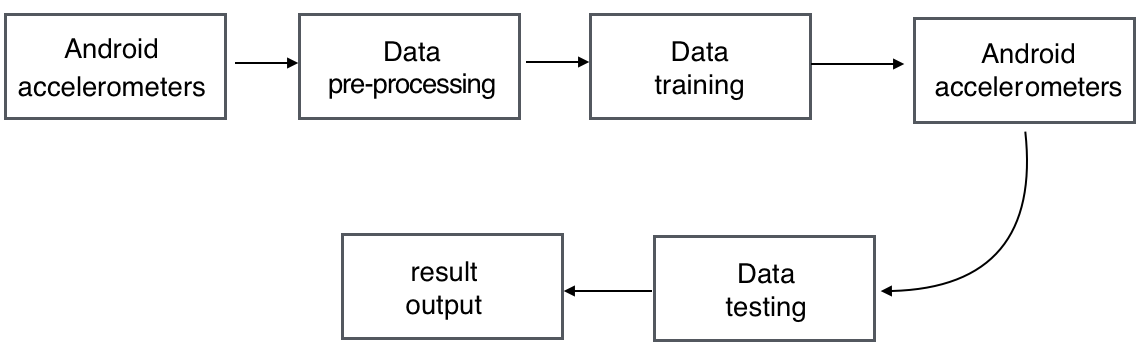
\includegraphics[width=0.5\textwidth]{system_overview}
\caption{System Overview}
\label{fig:system_overview}
\end{figure}

% 5. System Design
\section{System Design}

% 5.1 Model
\subsection{Model}
There are mainly three models to choose:

\begin{itemize}
	\item All-user model: this model will reduce the the time of training period, we can collect data set ahead and have it trained provide the result as the base when a user starts to use the device, but it usually has the worst accuracy, because even based on general or average training cases, the water drinking movement is a personal specific character a user has, therefore there are many trivial difference between users.
	\item Personal model: As we describe that the gesture is treated as a personal one, this personal model has the best accuracy. The drawback is it will need a long period of time to get enough training data so as to reach a high accuracy.
	\item Hybrid model: hybrid model combines the all-user model and the personal model. It bootstraps from a general all-user model and grows with a personal model by using personal data. This model will reach an acceptable accuracy more quick than a personal model. But it would take longer than the personal model if it wants to reach a high accuracy.
\end{itemize}

For our to-be tracked movement is mainly personalized one, we choose to use a personal model\cite{LiKamWa:2013:MBM:2462456.2464449}.

% 5.2 Feature
\subsection{Feature}
We collect 190 sample points for one drinking movement for our test using the linear accelerator in the smart phone. Each point has three values: $x$, $y$, $z$, which stands for the acceleration force along the three axes (excluding gravity). We use the following formula to reduce the 3 dimensions to one dimension: $x^2+y^2+z^2$. After this operation, pass the data through a low pass to exclude the noise.

Then we compute the change value: for the $i^{\text{th}}$ point's value $samplePoint[i]$ and the $(i+1)^{\text{th}}$ point's value $samplePoint[i+1]$, the change value $changeValue[i]$ is $samplePoint[i+1] - samplePoint[i]$. There are totally 189 change values. We also compute the mean value standard deviation of the 190 sample points and add these two values into the list of the features. In the end we have 191 features for one drinking movement\cite{Jain}.

% 5.3 Algorithm
\subsection{Algorithm}
We pick three algorithms that may fit to our requirement of recognizing the drinking movement: J48, RBFNetwork and MultiplayerPerceptron\cite{Weka}.

J48: J48 is a classifier in Weka. It is an implementation of C4.5 algorithm and use decision tree. A decision tree is a decision support system that implements tree-like graph decisions and their possible after-effect, including chance event results, resource costs, and utility. It is also used to learn a classification function which concludes the value of a dependent attribute (variable) given the values of the independent (input) attributes (variables). This verifies a problem known as supervised classification because the dependent attribute and the counting of classes (values) are given[8].

RBFNetwork: RBFNetwork is a class that implements a normalized Gaussian radial basis function network. It uses the k-means clustering algorithm to provide the basis functions and learns either a logistic regression (discrete class problems) or linear regression (numeric class problems) on top of that. Symmetric multivariate Gaussians are fit to the data from each cluster. If the class is nominal it uses the given number of clusters per class.It standardizes all numeric attributes to zero mean and unit variance[3].

MultiplayerPerceptron: MultiplayerPerceptron is a classifier that uses back propagation to classify instances. This network can be built by hand, created by an algorithm or both. The network can also be monitored and modified during training time. The nodes in this network are all sigmoid (except for when the class is numeric in which case the the output nodes become un-thresholded linear units)[3].

As our experiment goes on, the result shows that the accuracy of the MultiplayerPerceptron is not quite stable. For one user it reach as high as 91\%, however for another user, it falls to as low as 50\%. Additionally. This algorithm has a high time cost issue. Therefore we would use the previous two algorithms and drop the last one.

% 6. Implementation
\section{Implementation}
The process of our experiment is:

\begin{enumerate}
	\item Acquire number of sample points
	\item Training
	\item Test
\end{enumerate}

First we test to see how many sample points we should get for each movement(Figure 1). We collect over 10 cases to test how many sample points it will record for the entire movement, Figure 2 shows some of them. We conclude the following statistics:
\begin{itemize}
	\item Short: 150 points (150~170)
	\item Mid: 170 points (170~190)
	\item Long: 190 points (>190)
\end{itemize}

% Figure 2
\begin{figure}[htbp]
\centering
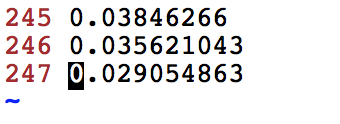
\includegraphics[width=0.2\textwidth]{acquire2}
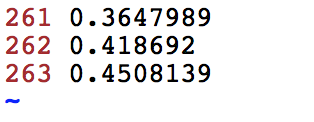
\includegraphics[width=0.2\textwidth]{acquire3}
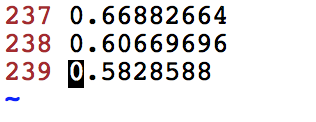
\includegraphics[width=0.2\textwidth]{acquire4}
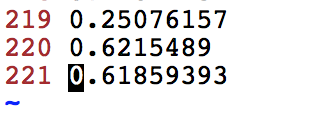
\includegraphics[width=0.2\textwidth]{acquire5}
\caption{Acquire number of sample points}
\label{fig:acquire}
\end{figure}

% 6.1 First Attempt
\subsection{First Attempt}
The first attempt of our experiment is to have 50 data as training set that are all positive movement, we say it is TRUE. Then each time we have a test case, no matter if it is predicted result is correct, we add it into the training set to let it grow in this way. Finally we have about 20 tests cases and all are included into the training set one by one. However, the accuracy of the predicted results is very bad, only about 40\%. The reason is that the test results do not have a regulation or correction. When we have a false positive of false negative result we still include it into the training set, which makes the set less accurate.

% 6.2 Second Attempt
\subsection{Second Attempt}
The second attempt of our experiment is to use a different accelerator, the gyroscope accelerator. However, since the movement does not require too much rotate on  the wrist, the data we get has little changes, then we would keep focusing on using the linear accelerator.

% 6.3 Modification
\subsection{Modification}
For the first attempt, we simply do not add the test cases into the training data set, instead, we could let user to correct the test case first and then let user choose to add it into the training set. This would be a future work of our experiment. Now we will use the fixed 50 data as the training set. Also, we decide to add negative movement data, that is FALSE data, into the training set instead of just all TRUE data. We will use 25 TRUE data and 25 FALSE data to build the training set.

For the second attempt, for now we do not consider using the second accelerator.

% 6.4 Data Pre-processing
\subsection{Data Pre-processing}
After collecting the data, we use the software with GUI window provided by Weka to have a pre-processing on the data. The Figure 3 shows the pre-processing of J48, and the Figure 4 shows the pre-processing of RBFNetwork:

% Figure 3
\begin{figure}[htbp]
\centering
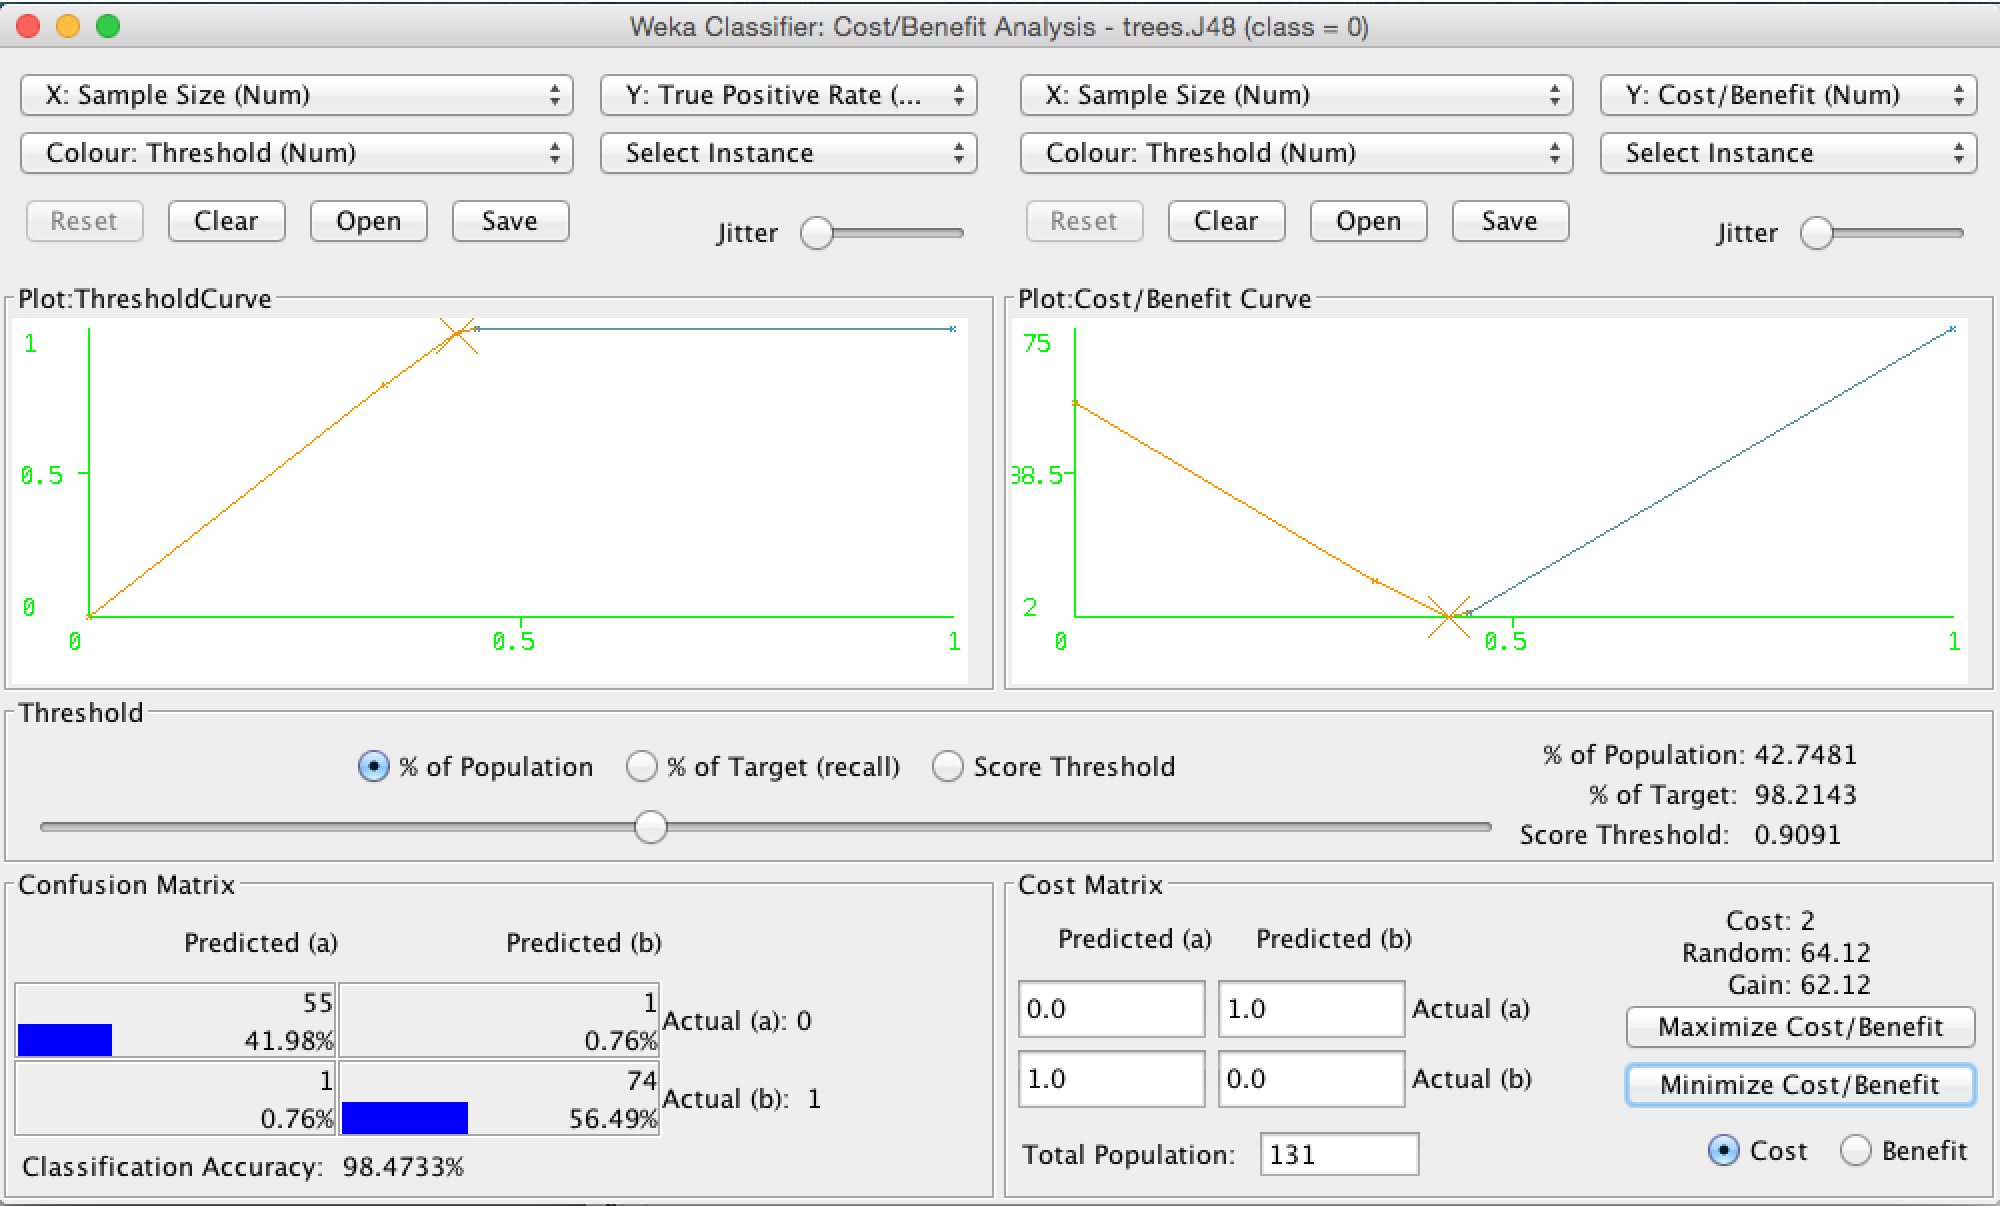
\includegraphics[width=0.5\textwidth]{pre_j48}
\caption{J48 Pre-processing}
\label{fig:pre_j48}
\end{figure}

% Figure 4
\begin{figure}[htbp]
\centering
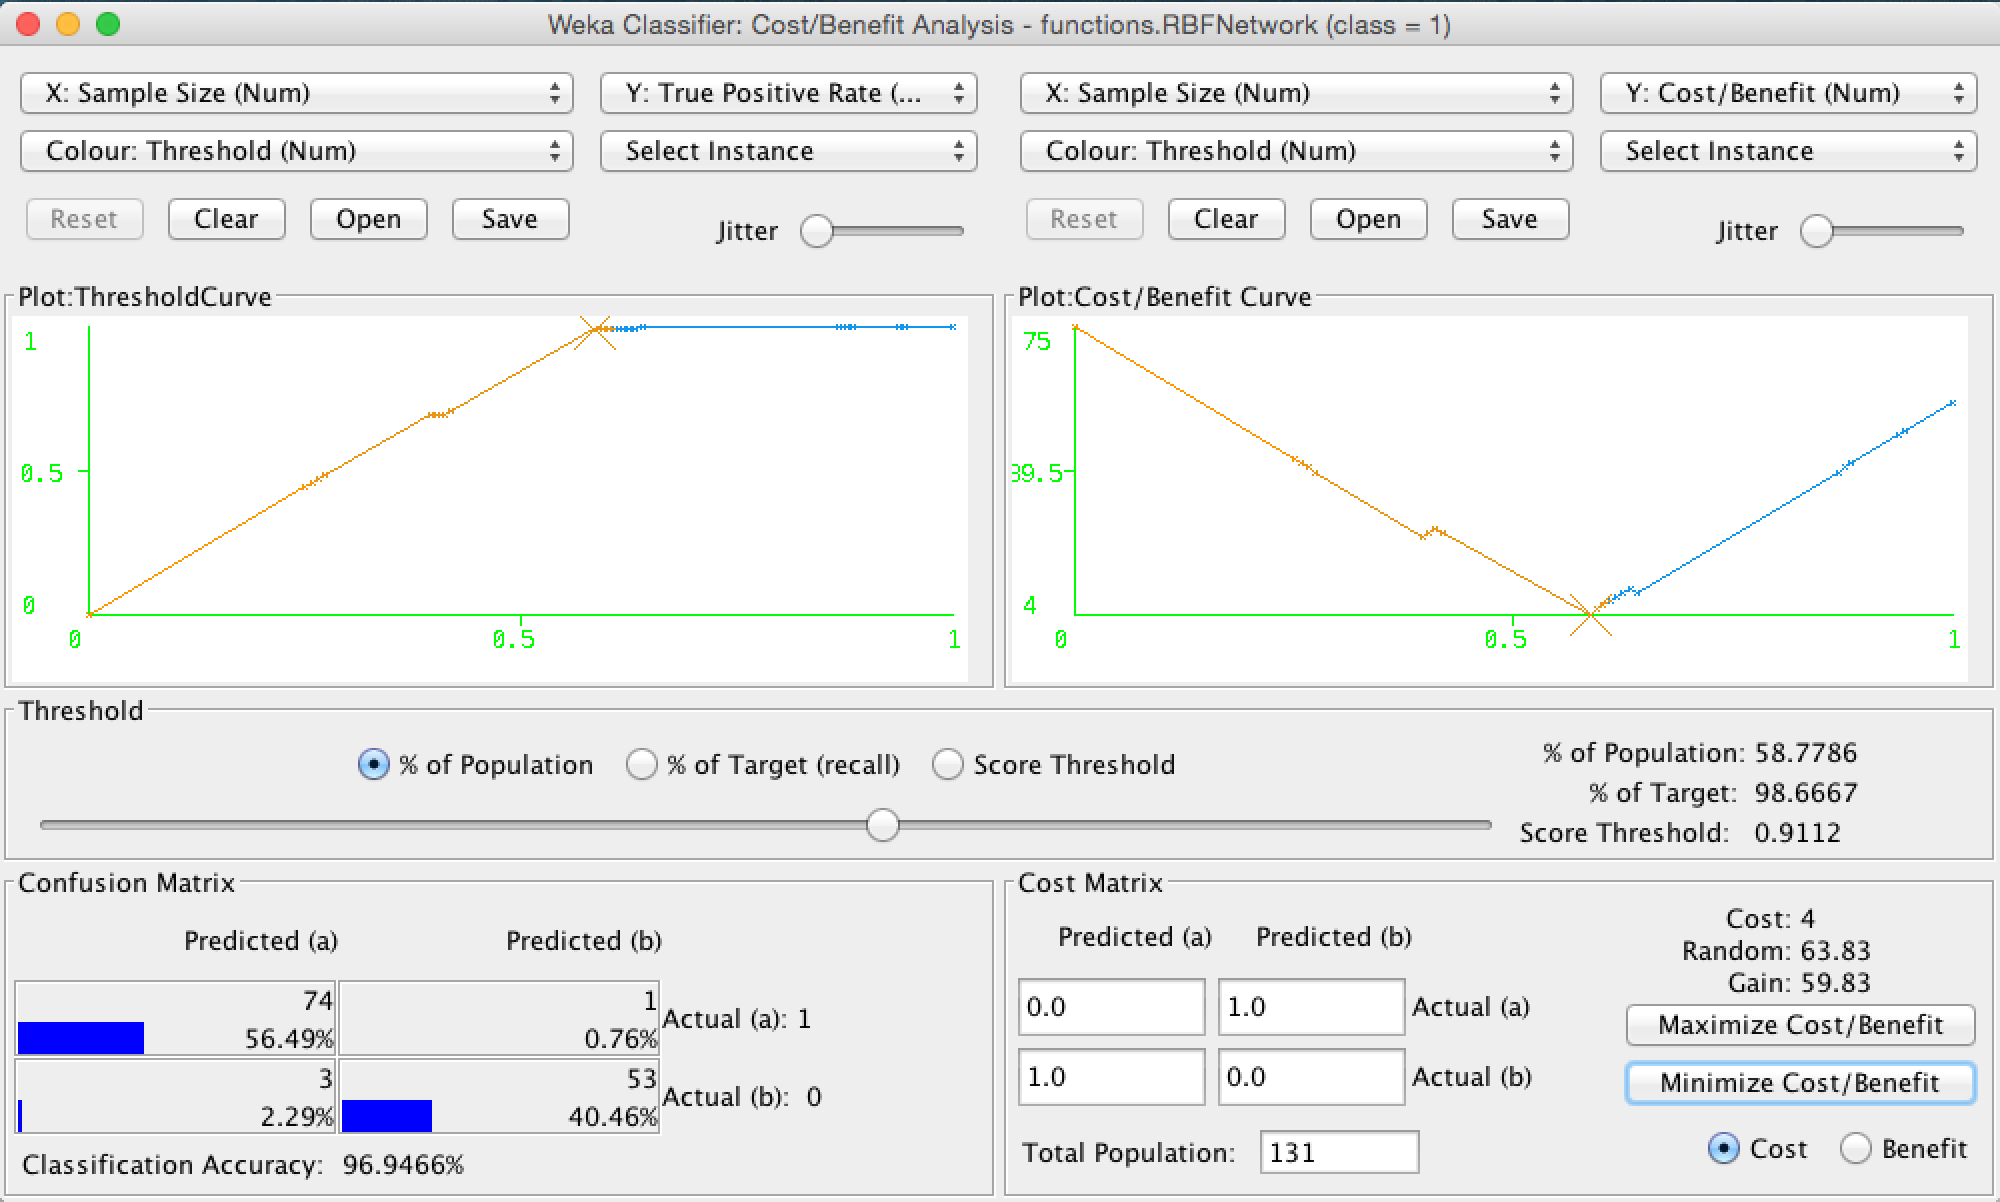
\includegraphics[width=0.5\textwidth]{pre_rbfnetwork}
\caption{RBFNetwork Pre-processing}
\label{fig:pre_rbfnetwork}
\end{figure}

The graph describes that the classification accuracy of both algorithms is high enough that the data collected is able to be used to have the training. Also from the axis we can tell that when the training uses over 60\% of the amount of the data, its classification accuracy is already close to 100\%. That means the amount of the training data is enough. 

% 6.5 Training
\subsection{Training and Test}
By using the Android app we can collect the data and start training as well as test. We collect the training data set with 130 samples (75 TRUE, 55 FALSE) Test data set: 44 cases (27 TRUE, 17 FALSE). Here is the comprehensive test results of J48 and RBFNetwork for one user (Figure 5 and Figure 6).

% Figure 5
\begin{figure}[htbp]
\centering
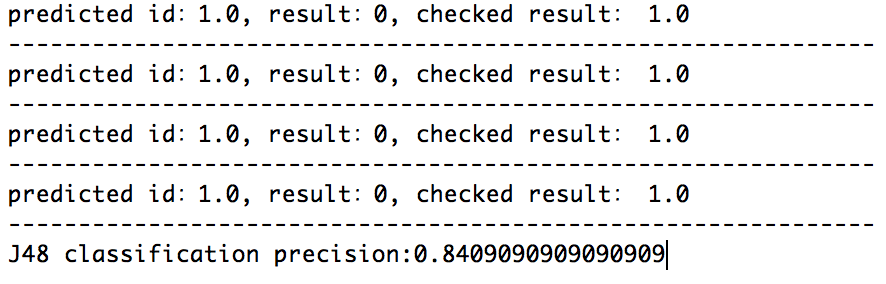
\includegraphics[width=0.5\textwidth]{result_j48}
\caption{J48 Result}
\label{fig:result_j48}
\end{figure}

% Figure 6
\begin{figure}[htbp]
\centering
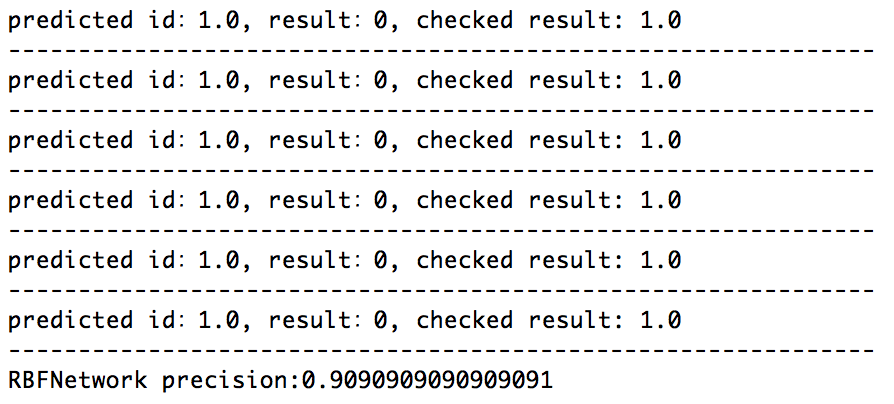
\includegraphics[width=0.5\textwidth]{result_rbfnetwork}
\caption{RBFNetwork Result}
\label{fig:result_rbfnetwork}
\end{figure}

The accuracy of J48 comes: accuracy is 84\%, false positive is 0, false negative is 16\%. The accuracy of RBFNetwork comes: accuracy is 91\%,  false positive is 0, false negative is 9\%. Both of the results meet our expectation. We give out some more results of an additional user. The raining data set is 115 samples (75 TRUE, 40 FALSE) ,test data set is 50 cases (25 TRUE, 25 FALSE). The accuracy of J48 comes: accuracy is 90\%, false positive is 8\%, false negative is 2\%. The accuracy of RBFNetwork comes: accuracy is 80\%,  false positive is 20\%, false negative is 0.

% 7. Evaluation
\section{Evaluation}

% 7.1
\subsection{Decision Tree Compare}
The following Figure 7 is the Decision Tree compare of the first user and the second. From the graph, we can tell that the first user has to use more features to make classification  than the second user. They have different characteristic gesture of the drinking movement. For the second user, the reason for the such a single decision tree to be generated is that, this user has quite the same track when he/she is do that movement\cite{Korting}.

% Figure 7
\begin{figure}[htbp]
\centering
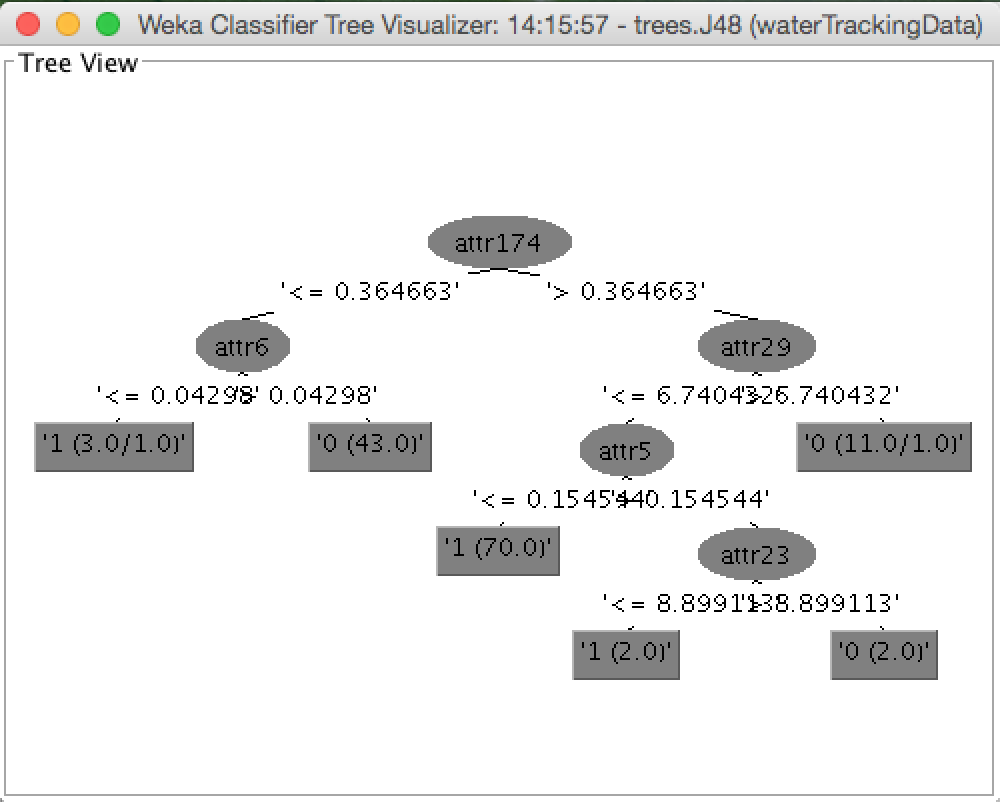
\includegraphics[width=0.4\textwidth]{j48_tree_m}
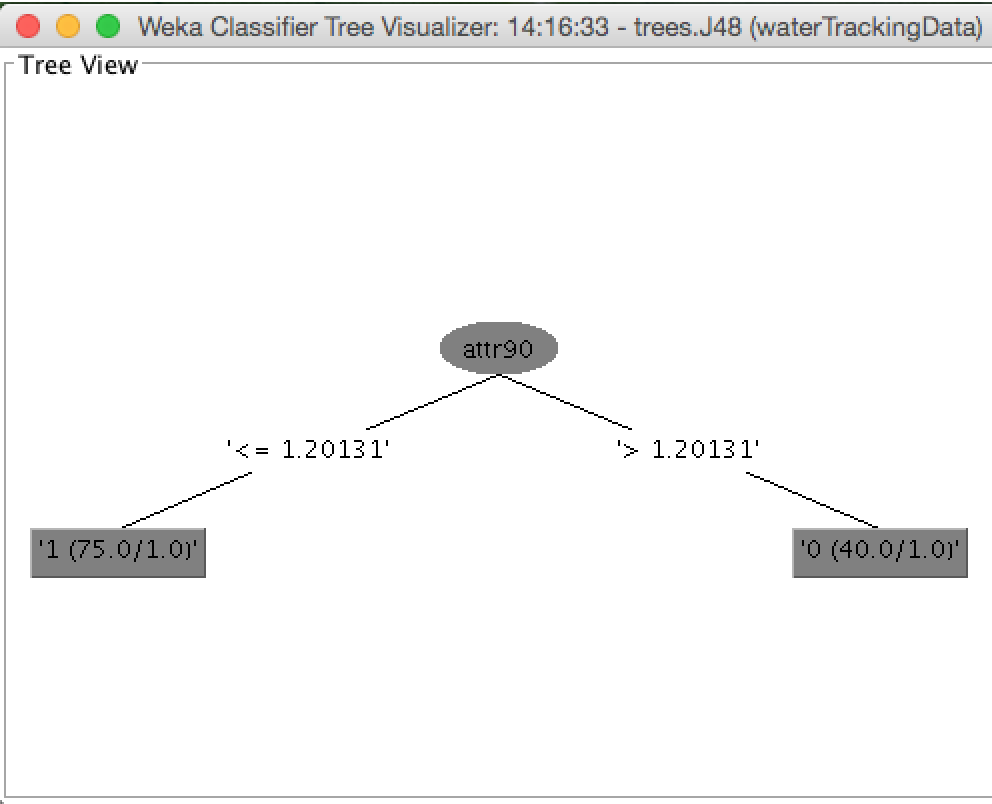
\includegraphics[width=0.4\textwidth]{j48_tree_f}
\caption{Decision Tree Compare}
\label{fig:j48_tree}
\end{figure}

% 8. Android Application
\section{Android Application}
With this Android application, we can collect training data into a training file stored in the smart phone and use it for further prediction(Figure 8). After the training phase, the app then starts to make the prediction and show the result to the user (Figure 9). This simple yet practical Android app is build with the J48 algorithm inside. It can simply run the training without any high time cost\cite{androiddeveloper}.

% Figure 8
\begin{figure}[htbp]
\centering
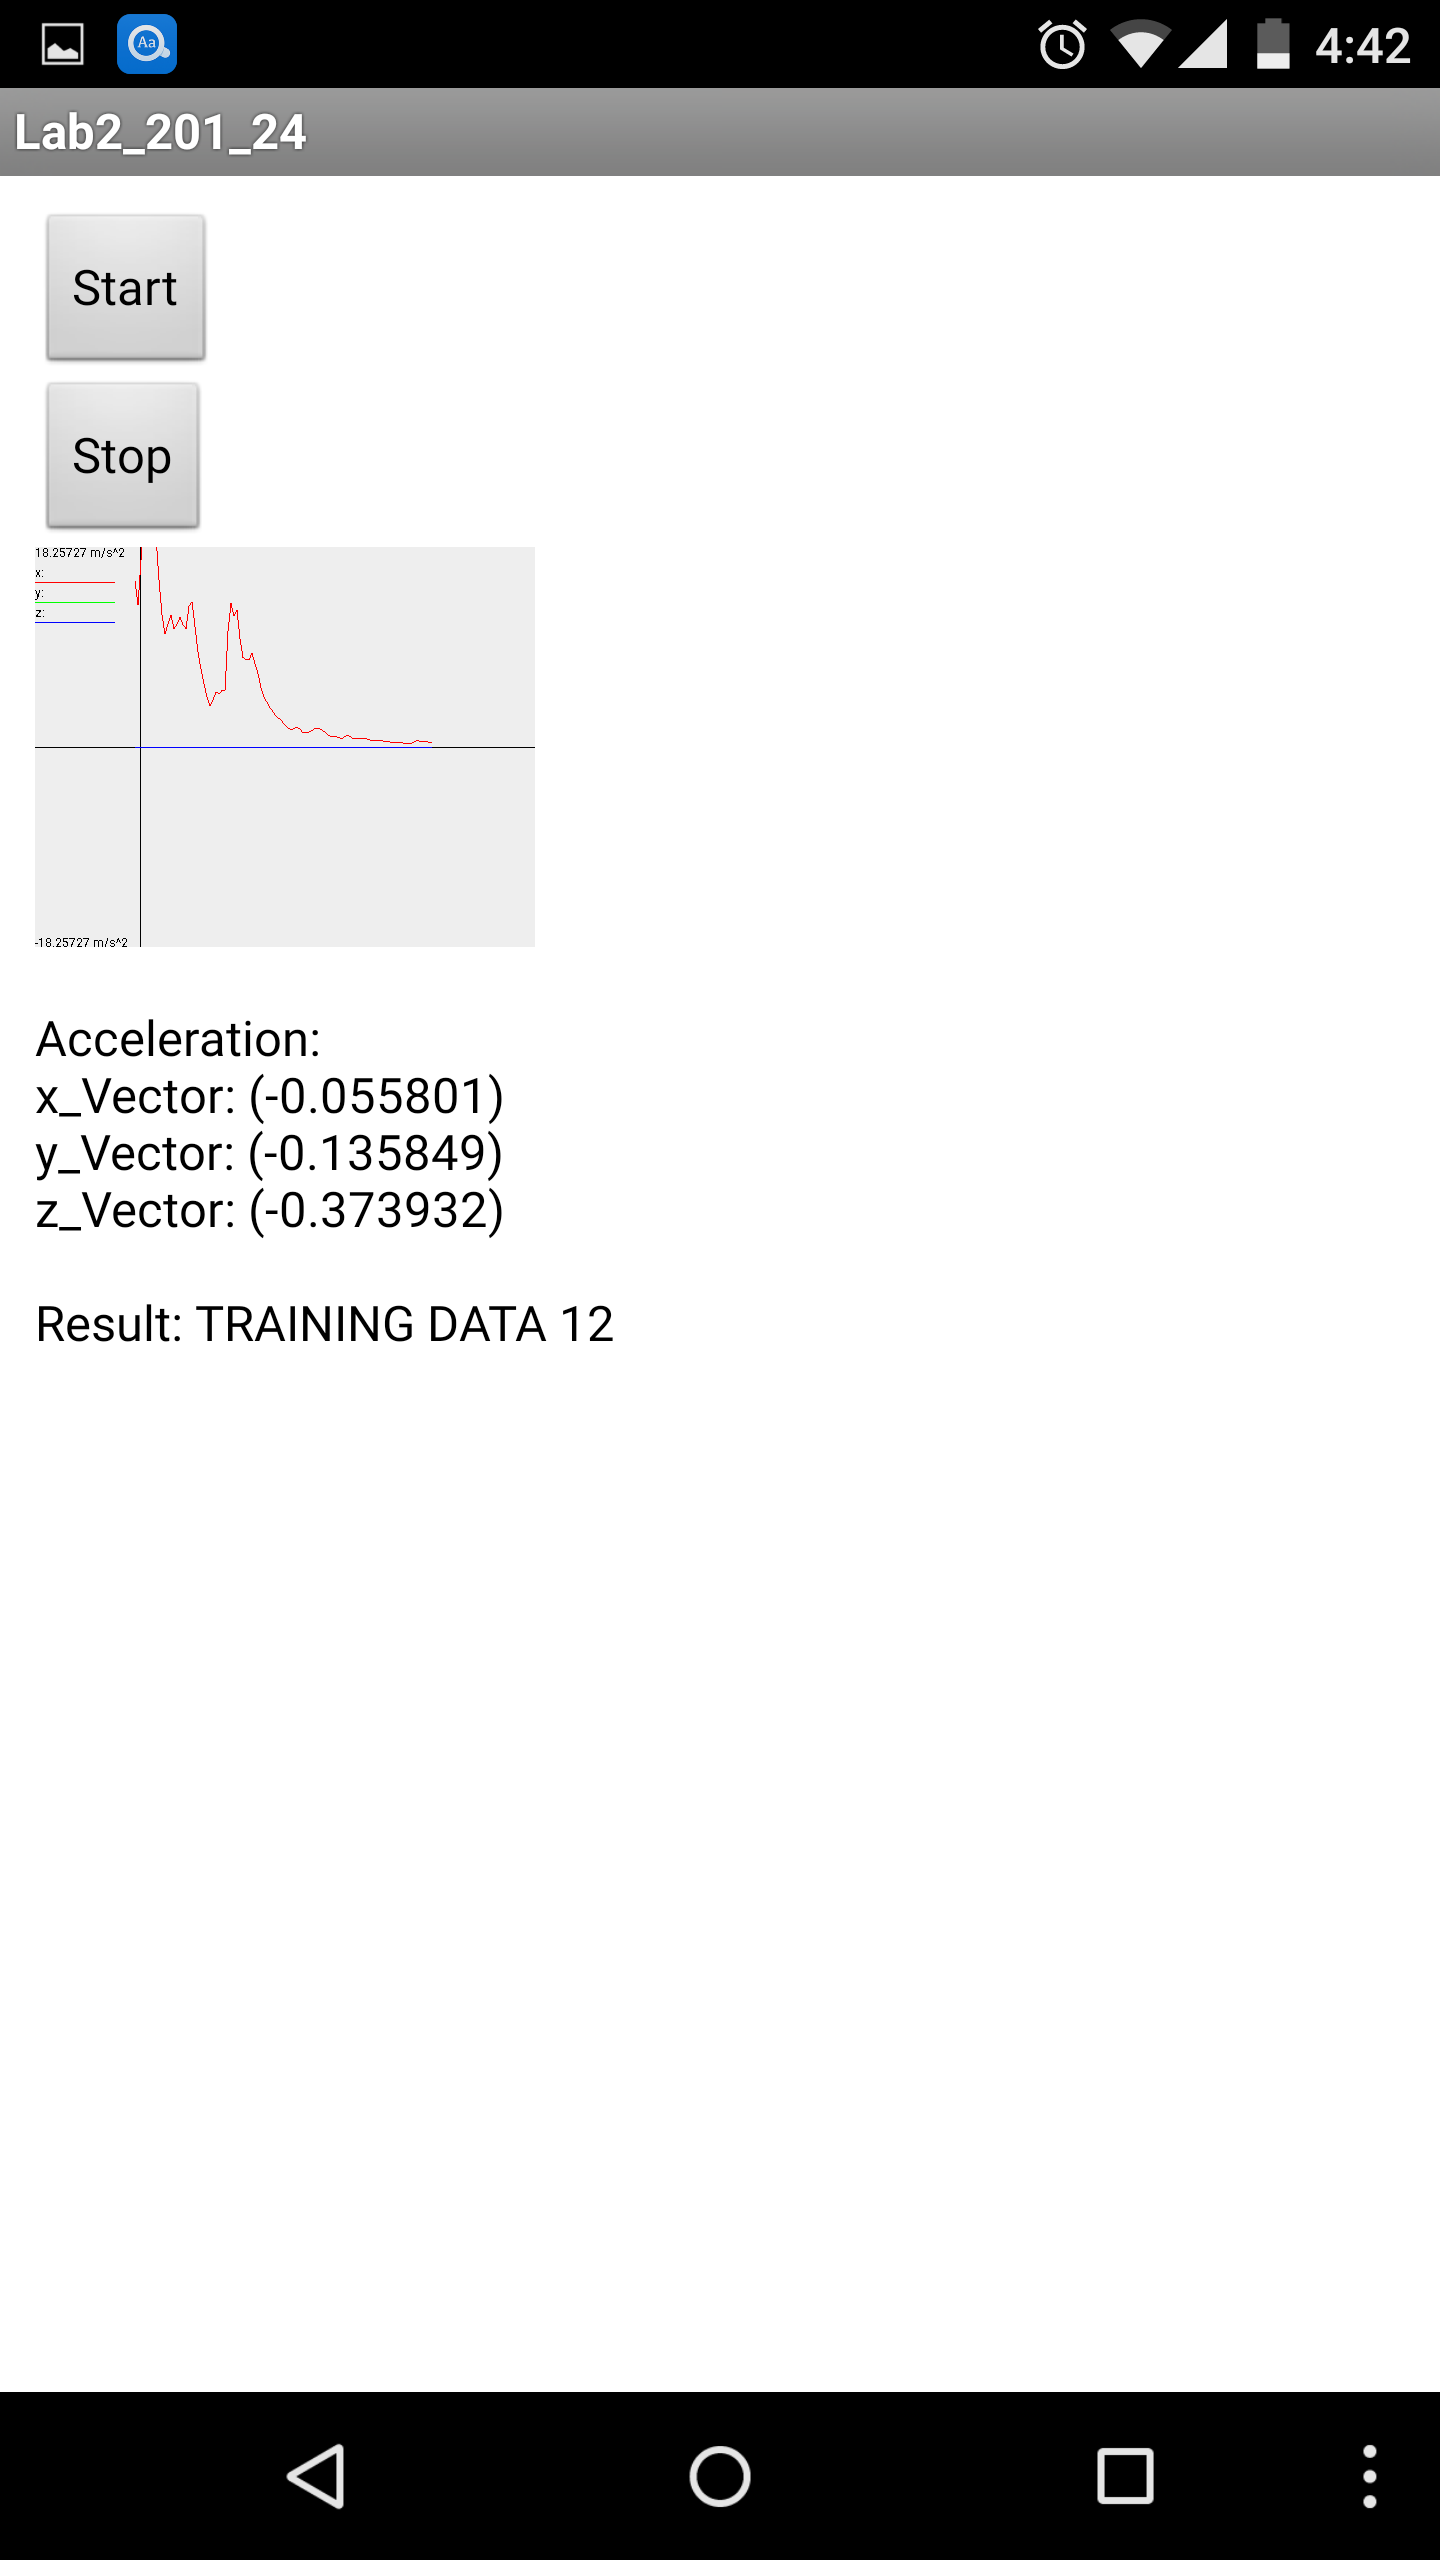
\includegraphics[width=0.2\textwidth]{app_training}
\caption{Android Application Training}
\label{fig:app_training}
\end{figure}

% Figure 9
\begin{figure}[htbp]
\centering
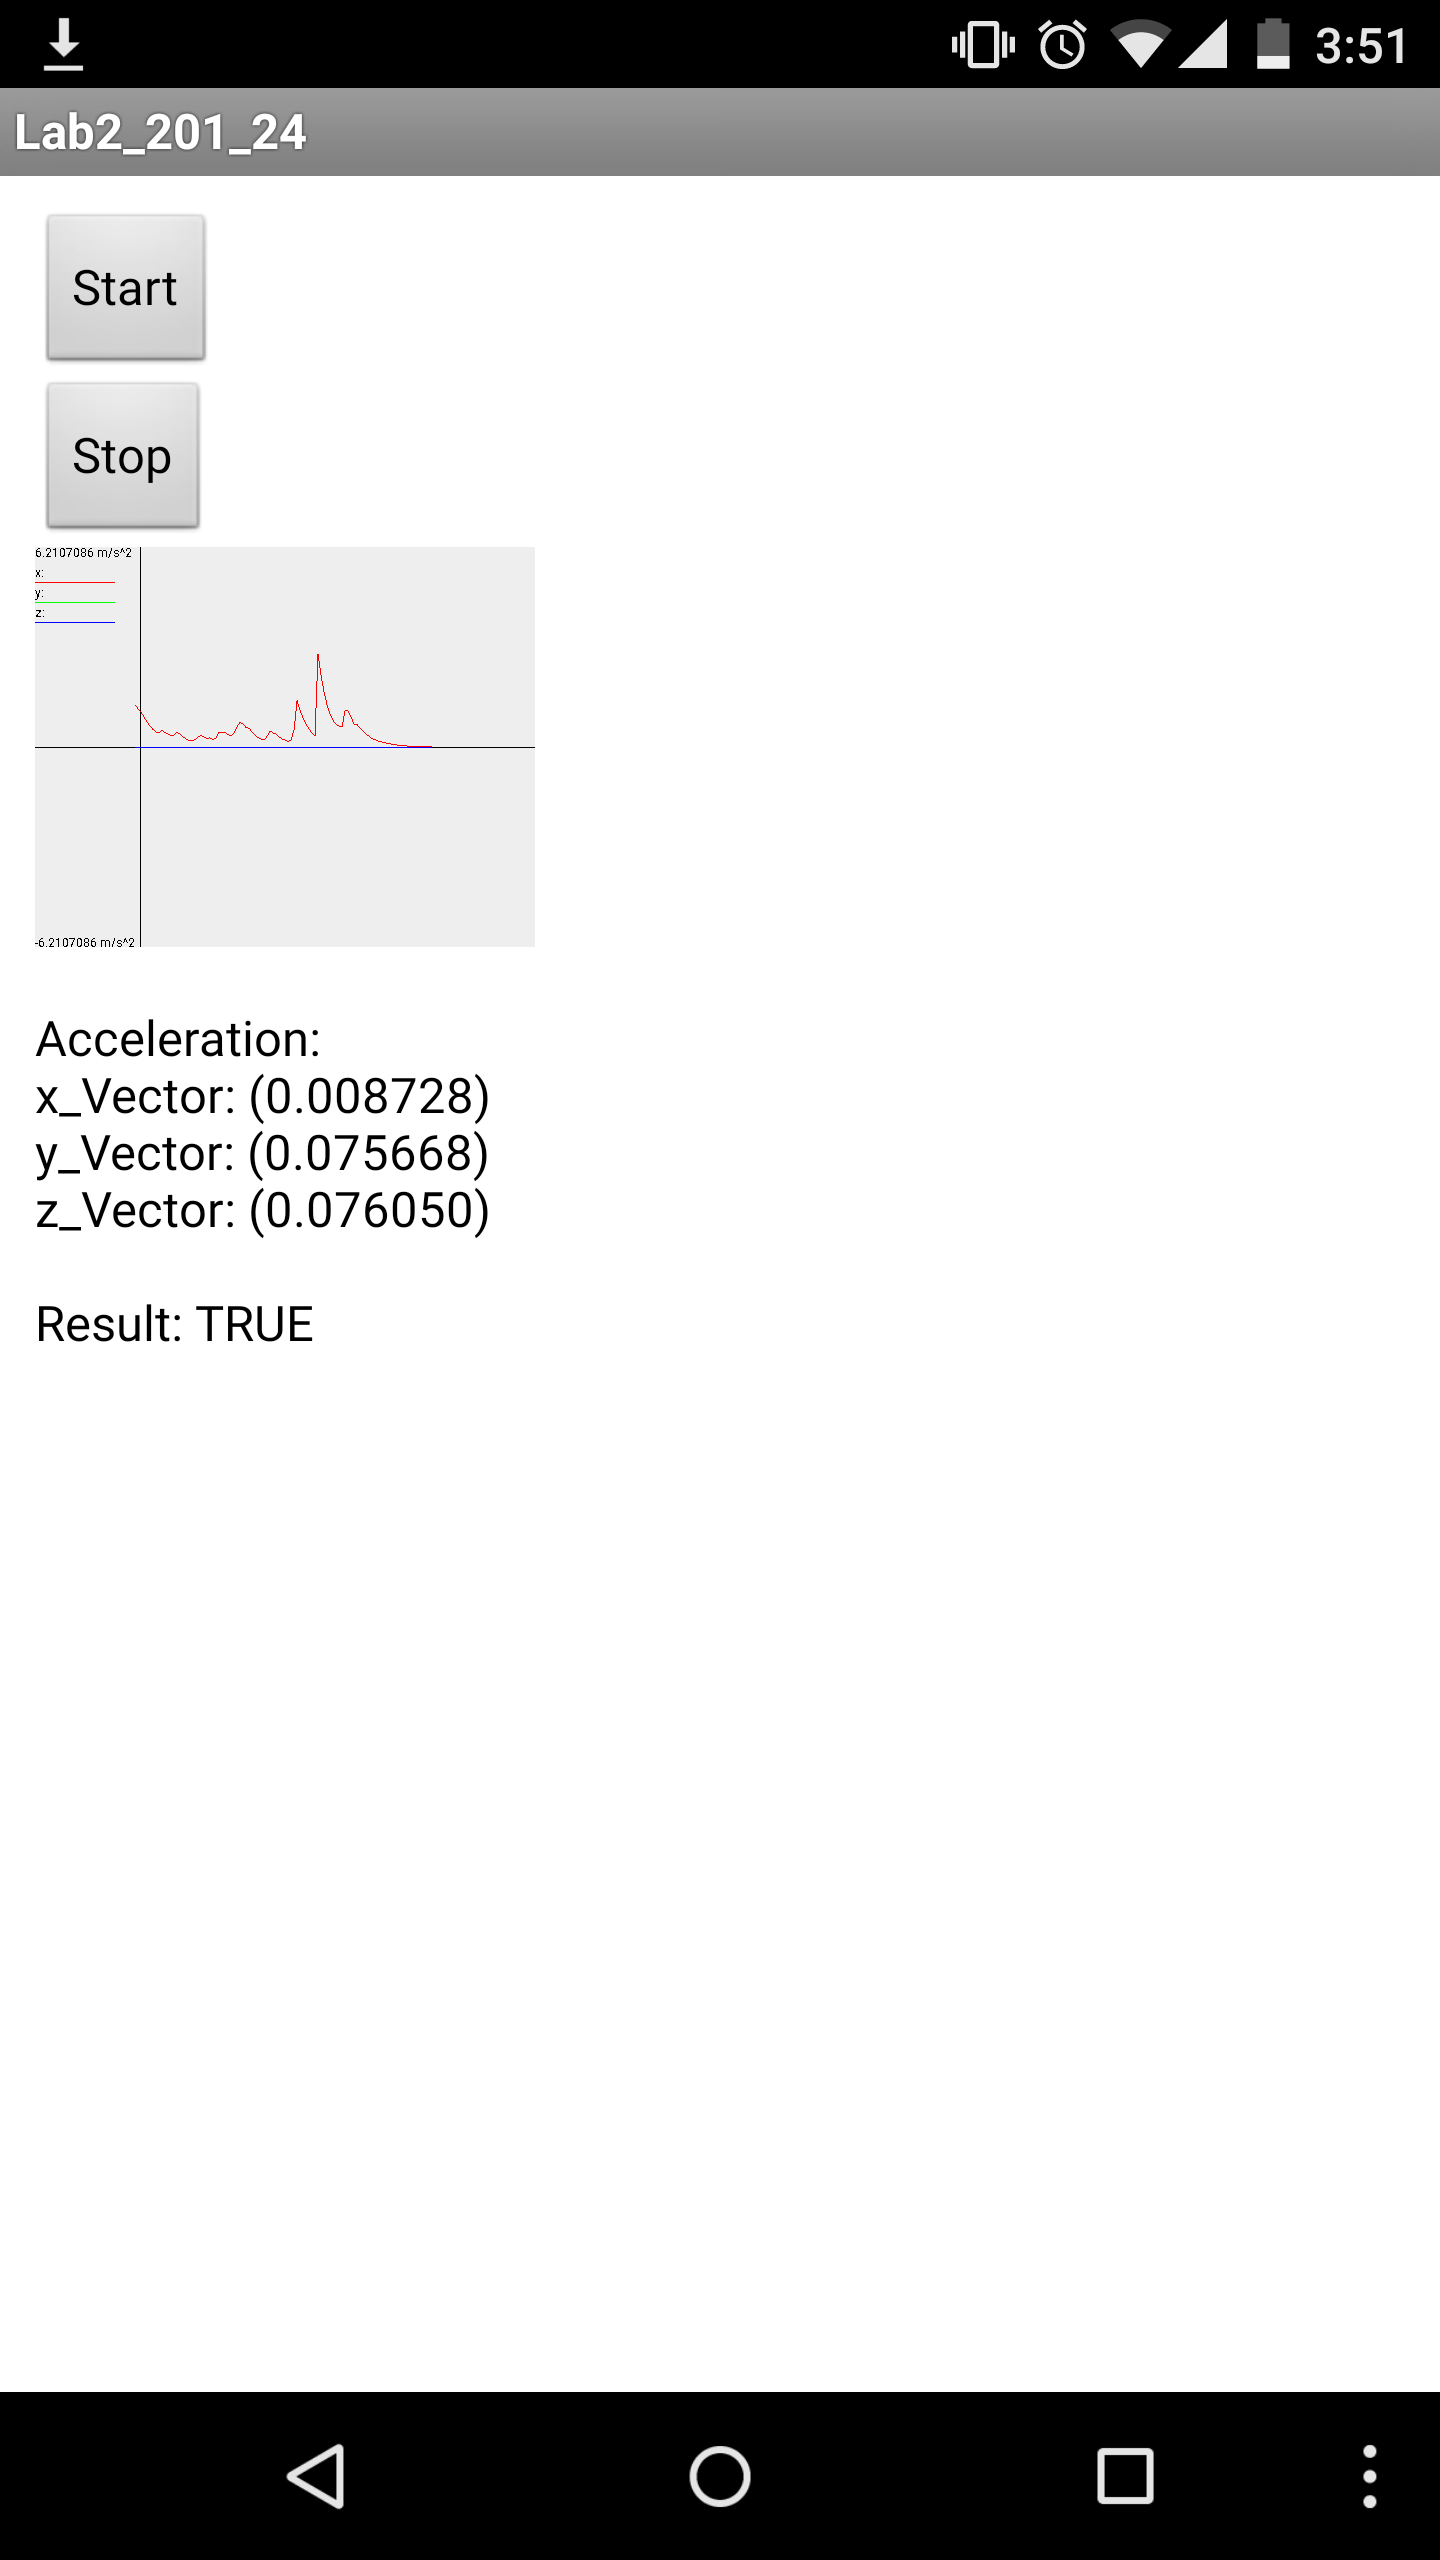
\includegraphics[width=0.2\textwidth]{app_test}
\caption{Android Application Test}
\label{fig:app_test}
\end{figure}

% 9. Future Work
\section{Future Work}

% 9.1
\subsection{More test data, less training data}
The good algorithm always have high efficiency. It can use less training data and output the more accuracy results. Our experiments have more training data rather than test data which is not proper.

% 9.2
\subsection{More raw data and proper feature extraction}
Feature extraction by normal machine learning algorithm is also lacking in our experiments. After acquiring more raw data from other Android phone's accelerators, we could use more mathematical and practical way to extract the feature such as slide time window to do the feature extraction.

% 9.3
\subsection{Energy consuming}
Energy consuming is also an important issue in our paper. One way to solve the problem is to pre-detect the action of phone. Such as in the middle of the obtaining the data. We could have low sampling rate in high-like not drinking action while high sampling rate in more like the drinking water action.

% 9.4
\subsection{Time sequence rather than movement based data}
Our method just sample the raw data from one action. In the future, we could have one day data and split with actions. After that we could have one day data and process the data thus we could have the drinking time one day one time with better user experience.

% 10. Conclusion
\section{Conclusion}
We have present the design, implementation and evaluation of our system. A demo for our movement detection. It use linear accelerator of Android phone to acquire the raw data and use Weka algorithm such as J48 and RBFNetwork to train and test the raw data after rough processing with mathematical way processing. Then the Android phone can output the result in real time. The accuracy of the result is about 90\% in our experiment. 


% References
\bibliographystyle{unsrt}
\bibliography{cs557_project_paper}

\end{document}
% END
